\section{\name Attacks}
\label{sec:attack}

As with conventional correlation attacks, an attacker must observe
traffic that is both entering and exiting
the Tor network; in contrast to threat models from previous work, we
incorporate DNS instead of only
TCP traffic.
Figure~\ref{fig:attack-scenario} illustrates our correlation attack; it requires the
following building blocks:
\begin{figure}[t]
	\centering
	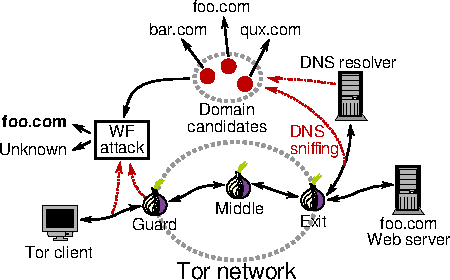
\includegraphics[width=0.8\linewidth]{figures/attack-scenario.pdf}
	\caption{An overview of the \name attack.  An adversary must monitor
		both ingress (encrypted Tor traffic) and egress (DNS request) traffic.
		A AS-level adversary between the
		client and its guard monitors ingress traffic.  The same adversary
		monitors egress traffic between the exit and a DNS server, or the DNS
		server itself.  Both ingress and egress traffic then serve as input to the
		\name attack.}
	\label{fig:attack-scenario}
\end{figure}

\begin{itemize}
    \item \emph{Ingress sniffing:} An attacker must observe traffic that is
		entering the Tor network.  The attacker can operate on the network level,
		as a malicious ISP or an intelligence agency.  In addition, the
		attacker can operate on the relay level by running a malicious Tor guard
		relay.  In both cases, the attacker can only observe encrypted
		data, so packet lengths and
		directions are the main inputs for website fingerprinting~\cite{Panchenko2016a}.
    \item \emph{Egress sniffing:} To observe both ends of the communication, an
		attacker must also observe egress DNS traffic.  We expect the adversary
		either to be on the path between exit relay
		and a DNS server or to run a malicious DNS
		resolver or server.  An attacker may also run an exit relay,
		but in this case, conventional end-to-end correlation
                attacks are equally effective as those we describe here.
\end{itemize}
We combine a conventional website fingerprinting attack operating on traffic
from ingress sniffing with
DNS traffic observed by egress sniffing, creating \name attacks. Our attacks
correlate the web\emph{sites} observed by the website fingerprinting attack in
ingress traffic with
the web\emph{sites} identified from DNS traffic. Next, we describe how we
simulate the DNS traffic from Tor exits, how we map DNS requests to websites,
and finally present our two \name attacks.

\subsection{Approximating DNS traffic from Tor exits}
\label{sec:attack:sim}

We first investigate the DNS traffic that Tor's exit relays send.
There are no logs of outgoing traffic
from Tor exit relays available to us, and ethical considerations kept us
from trying to collect them (\eg, by operating exit relays and recording
all the outgoing traffic). We therefore opt to approximate the DNS traffic
emerging from Tor exit relays by \first building a model of typical Tor
users' website browsing patterns, \second collecting a minimally invasive
dataset of DNS traffic, and \third accounting for the effects of DNS caching.

\subsubsection{Modeling which sites Tor users visit}
\label{sec:attack:pop}

We first build a model to approximate {which websites} Tor users visit.
Currently, there are about 173 million active
websites~\cite{numberofwebsites}; the Alexa ranking~\cite{alexatop1k}
gives insights into their popularity based on the browsing behavior of
a sample of all Internet users. The distribution of the popularity of
these websites has previously been fit to a power-law distribution based
on the rank of the
website~\cite{DBLP:journals/network/MahantiCMAW13,ClausetSN09,AliS07}.
For the pageview numbers of the Alexa top 10,000 websites, we found a
power-law distribution to be a good fit as neither a log-normal nor a
power-law distribution with exponential cutoff (truncated power-law
distribution) offered significantly better fits.
We used the Python {\tt powerlaw} package~\cite{power-law} for fitting and
picked a power-law distribution with an $\alpha$ parameter of about $1.13$.
When varying the fitting parameter $x_{min}$ that determines beyond which
minimum value the power-law behavior should hold in the provided data, we can
get different $\alpha$ values. We made a conservative choice of picking this
smaller $\alpha$ value as it underestimates the popularity of popular websites
and therefore is worse for the attacker.\footnote{Alexa's page-view numbers
ignore multiple visits by the same user on the same day (see
\url{https://support.alexa.com/hc/en-us/articles/200449744}), so the ranking
might be slightly off when modelling website visit patterns.}
Thus, we use a power-law distribution to model which websites are
visited by Tor users. This might overestimate the popularity of
higher-ranked websites, because Tor users might be visiting less popular
websites, such as websites that are censored in different parts of the
world more often than a typical Internet user. We will discuss the
implications of our model for browsing behavior later.

\subsubsection{Modeling how often Tor users visit each site}
\label{sec:load-freq}
% phw's numbers extrapolated
Next, we determined how many websites Tor users visit in a certain time span.
We approximated this number by setting up an exit relay whose exit policy
included only ports 80 and 443, so our relay would only forward web traffic.  We
then used tshark to capture the timestamps of DNS requests---but no DNS
responses.  We made sure that our tshark filter did not capture packet payloads
or headers, so we were unable to learn what websites Tor users were visiting.
In addition, we patched {\tt tshark} to log timestamps at a five-minute
granularity. The coarse timing granularity allows us to publish this
dataset with minimal privacy implications;
Section~\ref{sec:ethics} discusses the ethical implications of this
experiment in more detail.  We ran the experiment for approximately two weeks
from May 15, 2016 to May 31, 2016, which allowed us to determine the number of
DNS requests for 4,832 five-minute intervals.
Figure~\ref{fig:dns-reqs} shows this timeseries.

\begin{figure}[t]
	\centering
	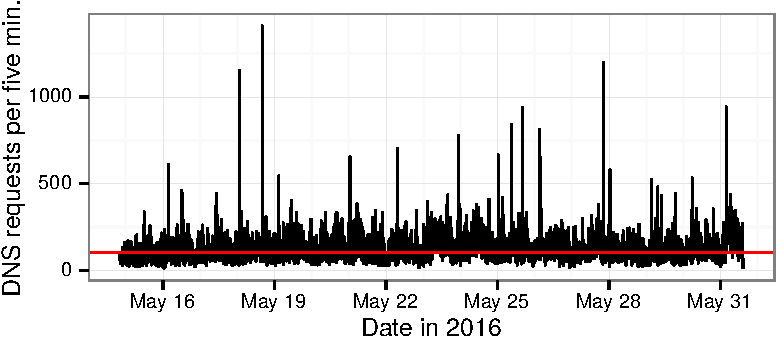
\includegraphics[width=\linewidth]{figures/dns-reqs.pdf}
	\caption{The number of DNS requests per five-minute interval on our
	exit relay.  Using a privacy-preserving measurement method, we only
	determined approximate timestamps and no content.  The red line at $y = 105$
	illustrates the median of the distribution.}
	\label{fig:dns-reqs}
\end{figure}

We then interpolate these numbers to all Tor exit relays based on the published
bandwidth statistics of all Tor exit relays. We found our exit relay to have an
average of 238.6 outgoing DNS requests per ten minutes during a two-week period.
We configured the exit relay to only allow port 80 and 443 during the time
of the measurements to avoid counting DNS requests from protocols other than
HTTP and HTTPS. % was mentioned above already, should we remove that here or keep for clarity?
From DNS statistics of the Alexa top one million websites (see
Section~\ref{sec:dns2site}) we know that one website visit causes outgoing DNS requests for about 10.3 domains on average
(assuming a power-law distribution of site popularity as described above and
taking into account tor caching pending DNS requests, ensuring that multiple
requests sent by clients for the same domain name only result in one outgoing request
by the exit).
This means that we had an average of about 23.2 website visits per ten
minutes on our exit relay. We can scale this number up to the whole Tor
network using the self-reported bandwidth information from Tor exit
relays collected in the ``extra-info'' descriptors available on
CollecTor~\cite{collector} and estimate the number of website visits on
each of the about 1,200 exit relays active at that time. The resulting average
total number of websites visited through the Tor network is about 536,000
websites per ten minutes.

Recently, Jansen and Johnson~\cite{jansen-ccs2016} measured the average
number of active web (port 80 and 443) circuits in Tor to about 700,000 per ten
minutes.\footnote{This number comes from a preprint kindly
shared by the authors and might change in the final version.}
In the Tor Browser Bundle (TBB), the browser builds one circuit per
website entered in the URL bar. How long the circuit remains active depends on
TBB settings (primarily MaxCircuitDirtiness currently set to ten minutes) and how
long TCP streams in the circuit are active: as long as at least one stream is
active, the circuit remains active. The number of active circuits serves as an
upper bound for the number of websites visited over Tor: visiting different
pages of a website will use the same circuit, and visiting a new website will
construct a new circuit. Users visiting several pages of a website and websites
with long-lived connections, like Twitter and Facebook with continuously
updating feeds,
all lower the number of websites visited in Tor relative to the number of active
circuits. In later sections we revisit the implications of our estimates by
scaling the Tor network to ten-times its estimated size.

\subsubsection{Modeling the effects of DNS caching}
To analyze which DNS requests the adversary can see, we need to
take caching of DNS responses into account. We ignore client-side DNS
caching since it is disabled by default, as described in
Section~\ref{sec:background}.
% From Tobias: I manually could not get Firefox to cache anything,
% not even between pageloads on the same site (went to kau.se, waited 20s,
% then clicked on a link: little tor client-side still got a DNS response
% from the exit for kau.se.)
On the exit relays, which perform DNS resolution on behalf of Tor clients, caching
is relevant, because the requests of all users connected to an exit
share the same cache. An exit
relay maintains its own DNS cache\footnote{See
\url{https://gitweb.torproject.org/tor.git/tree/src/or/dns.c}.} and enforces a
minimum TTL of 60 seconds and a maximum TTL of 30 minutes.\footnote{See
\texttt{dns\_clip\_ttl} in
\url{https://gitweb.torproject.org/tor.git/tree/src/or/dns.c}.}  We
refer to this as Tor's \emph{TTL clipping}. Due to a
bug in Tor that we identified\footnote{We redacted the link to the bug report to anonymize our paper
submission.},
% \url{https://bugs.torproject.org/19025}}
the TTL of all DNS responses are set to 60 seconds, which determines
the duration the responses are cached.

%\subsubsection{Sliding window approach to compensate for DNS caching}
% we ignore caching by having a window of X minutes
If a user of an exit relay requests the IP address for a domain name
that has been cached by the exit relay before (and the cache entry is
not expired yet), then the adversary will not be able to observe an
outgoing DNS request for this domain name. But the adversary can
recorded all DNS requests from the exit relay in the past $x$ seconds,
where $x$ is the maximum TTL value (that is, maintain a sliding window of
length $x$) to obtain a list of all possibly requested domain names at the
given point in time. A domain name that is requested by a client at the
given point in time is either cached or not. If it is
not cached, it will be observable as a new, outgoing DNS
request from the exit relay. If it is cached it must
have been resolved by the exit relay in the last $x$ seconds and will
therefore be in the sliding window.

We assume that an adversary applies this sliding window technique and
model the observable DNS data accordingly.
The attacker observes a fraction of Tor exit bandwidth
for a specific window length,
and together with our website visit frequency estimation
this triggers a number of website visits in our simulation.
For each visit event we randomly draw a website using the
power-law website popularity distribution described above and put its
DNS requests into the window. As we will see next, we do not need to
simulate or consider the fact that the observed fraction of Tor exit bandwidth
corresponds to many different exits with individual caches.

\subsection{Inferring website visits from DNS requests}
\label{sec:dns2site}

Given a sliding window of DNS requests, we investigate
how this information can help determine whether a user has visited a website of interest.
In April 2016, we visited the Alexa top one million websites five times
and collected all DNS requests generated by visiting each
website. We refer to the data collected for one visit as a \emph{sample}.
We performed these measurements in rounds from a university network, where
each round browsed all one million websites in a random order before visiting
the same website again. We used TBB~5.5.4
configured {\em not to browse over Tor}: TBB ensures that the browser behavior
is identical to a TBB user over Tor. Not using Tor bypasses
IP blacklists and CAPTCHAs triggered by IP addresses of
Tor-exits~\cite{Khattak2016a}.
Table~\ref{tab:dns-censor} shows the percentage of websites in our dataset that
risks censorship by CloudFlare or Akamai if collecting data over Tor, as
identified by Khattak \ea~\cite{Khattak2016a}. We also include Google,
which is prevalent in our dataset and
reportedly restricts access to Tor users (when searching).

\begin{table}[t]
	\renewcommand{\tabcaptext}{The percentage of websites on Alexa top-1 million websites using providers
	involved in censoring or restricting access from
        Tor~\protect\cite{Khattak2016a}.}
      \topcap{\tabcaptext}
	\centering
	\begin{tabular}{l r}
	\toprule
	\textbf{Description} & \textbf{Percentage} \\
	\midrule
	Website behind CloudFlare IP & 6.44 \\
	Domain on website uses CloudFlare & 25.81 \\
	Domain on website uses Akamai & 33.86 \\
	Domain on website uses Google & 77.43 \\
	\bottomrule
	\end{tabular}
        \bottomcap{\tabcaptext}
	\label{tab:dns-censor}
\end{table}

We collected 2,540,941 domain names over 60,828,453 DNS
requests. The dataset contains 2,260,534 domains that are unique to
a particular website; we call these domains {\em unique
  domains}. Unique domains are particularly interesting because a DNS
lookup to a unique domain during an HTTP session can identify that a
user has visited a specific website. Figure~\ref{fig:unique-domains} shows the
fraction of
sites with unique domains for websites up to Alexa top one million.
For 96.8\% of all sites on the Alexa top one million
there exists at least one unique domain.
Interestingly, more
popular websites are less likely to have a unique domain associated with
them: 43\% of Alexa top 100 have a unique domain compared to 96.8\% for
top one million. Above Alexa top 100 the fraction is erratic between
27\% to 41\%---why is not apparent---but for less popular sites from Alexa 100
and downwards the trend is clear.

Table~\ref{tab:dns-domains} shows statistics for the number of DNS domains per
website. At least half of the sites have ten domains per website where
two of them are unique, suggesting that many website visits can be
identified from a single DNS request.

\begin{figure}[t]
	\centering
	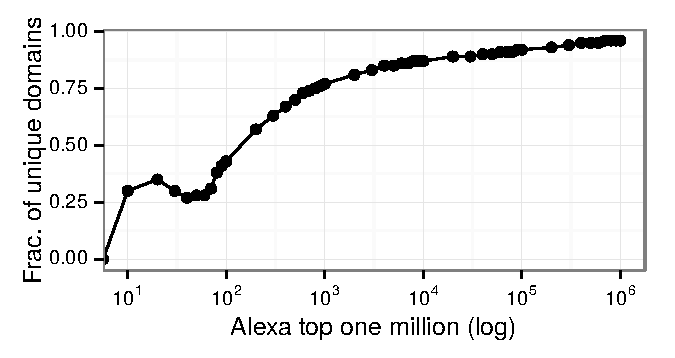
\includegraphics[width=0.9\linewidth]{figures/dns-unique-domains.pdf}
	\caption{The fraction of websites on Alexa top one million that have at least
	one unique domain. The vast majority of sites (96.8\%) have
        unique domains.
}
	\label{fig:unique-domains}
\end{figure}

\begin{table}[t]
	\renewcommand{\tabcaptext}{The median, mean, standard deviation, minimum and maximum number of
	DNS domains per website in the Alexa top 1 million. More than half of the
	sites have two DNS domains that are unique to that site.}
      \topcap{\tabcaptext}
	\centering
	\begin{tabular}{l r r r r}
	\toprule
	\textbf{DNS Domains} & \textbf{Median} & \textbf{Mean} & \textbf{Min} & \textbf{Max} \\
	\midrule
	per site & 10 & $12.2\pm11.2$ & 1 & 397 \\
	unique per site & 2 & $2.3\pm\phantom{0}1.8$ & 0 & 363 \\
	\bottomrule
	\end{tabular}
        \bottomcap{\tabcaptext}
	\label{tab:dns-domains}
\end{table}



To evaluate the feasibility of mapping DNS requests to websites, we
construct a na\"{\i}ve website classifier that maps the unique domains
in a set of DNS requests to the corresponding website that contains a
matching set of domains.  With five-fold cross-validation on our Alexa
top one million dataset (with five samples per site),
we consider a closed world and an open world.
In the closed world, the attacker can use samples
from all sites in training; in the open world, some sites
are unmonitored and therefore unknown (as per the fold).  The
closed-world evaluation yields 0.955 recall.  In the open-world
evaluation, we monitor the Alexa top 500,000 with five samples each and
consider 433,000 unmonitored sites.  The number of unmonitored sites is
determined by our power-law
distribution to represent a realistic base rate (for the entire Tor network)
for evaluating our classifier: on average, for sites on Alexa top 500,000
to be visited 2.5 million times there will be about 433,000 visits to sites
outside of Alexa top 500,0000.  Our classifier does not take into account the
popularity of websites.
The open-world evaluation yields a
recall of 0.947 for a precision of 0.984.  By accounting for the order
of requests, per-exit partitioning of DNS requests, TTLs, and website
popularity, we expect that classifying website visits from DNS requests
might be made even more accurate.
Further, a closed world is a realistic setting:
gathering requests made by all 173 million active websites on the
Internet is practical with modest resources.
We use the conservative open world results when simulating the Tor network and
the attacker's success in mapping DNS requests to websites.
Our results indicate that observing DNS requests in Tor is
largely equivalent to observing sites visited over Tor.

\subsection{Classifiers for \name attacks}

We use Wa-kNN from Wang \ea~\cite{Wang2014a} (described in
Section~\ref{sec:background}) and a list of sites derived from
observing DNS requests to implement two \name attacks:

\begin{description}
	\item[\texttt{ctw}] We ``close the world''
	on a Wa-kNN classifier that we modified to consider only the distance to
	observed sites when calculating the $k$-nearest neighbors.
	The classifier still considers the distance to all unmonitored sites.
	\item[\texttt{hp}] When Wa-kNN classifies a trace as a monitored site, confirm
	that we observed the same site in the DNS data (ensuring {\em high
	precision}). If not, make the final classification unmonitored.
\end{description}
\noindent
These approaches apply to any website fingerprinting attack. The
\texttt{ctw} attack increases the effectiveness of conventional website
fingerprinting attacks by making them more akin to a closed-world setting,
where websites have known fingerprints and often the world is of limited size.
Conceptually, the attack could also include
a custom weight-learning run---training only on observed sites---but our initial
results noted little to no gain, despite significant increases in
testing time.
We expect that this is due to the fact that some features of traffic traces are
more useful than others, regardless of the training data~\cite{kfingerprinting}.
The \texttt{hp} attack only produces a positive classification if both ingress
and egress traffic are consistent, simple but effective.
